\chapter{Lavorazioni non convenzionali}\label{chp:NonConvenzionale}
Sono caratterizzate dal fatto che non usano l'energia meccanica per modellare il materiale.
Dato questo, la durezza del materiale non costituisce un limite a tale problema. Per cui ci sono diverse possibilità anche per materiali non normalmente lavorabili.
Alla figura \ref{fig:NonConv} sono riportate le principali lavorazioni
secondo una classificazione in base all'agente tramite il quale si lavora.

\begin{figure}
\centering
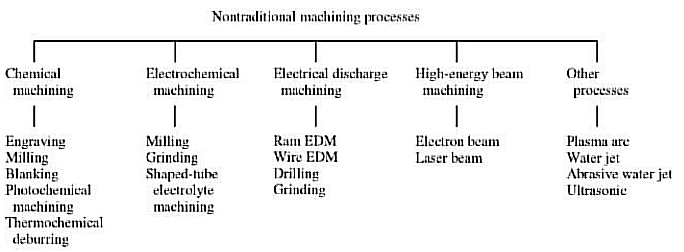
\includegraphics[width = \textwidth]{NonConv}
\caption{Classificazione lavorazioni non convenzionali}
\label{fig:NonConv}
\end{figure}

\begin{description}
\item[Attacco chimico] Si vuole rimuovere del materiale tramite azione chimica. Allora il problema non è più come togliere il materiale, piuttosto controllarla.
\item[Elettroerosione] Si sfrutta il movimento degli atomi per separarli dal lavorato.
\item[Scarica elettrica] Si sfrutta un arco elettrico per separare il materiale. Se ne era già parlato per la generazione delle polveri per la sinterizzazione
\item[lavorazioni ad alto contenuto energetico] Si parla di trasmettere elettroni ad alta energia per la separazione del materiale.
\item[Altre tipologie] in cui si includono il taglio ad acqua (anche se potrebbe rientrare tra le tecniche abrasive), lavorazioni ad ultrasuoni ecc\dots
\end{description}

Di solito sono lavorazioni realizzati nelle fasi finali della produzione.

\section{Lavorazioni chimiche}
Si provoca una corrosione controllata sul materiale da lavorare. Si proteggono le superfici che non si vuole corrodere detta \emph{maschera}, mentre le parti che devono essere rimosse vengono esposte all'ambiente corrosivo.
Perciò il metallo viene convertito in un composto solubile che rimarrà nell'attaccante corrosive.

Alla figura \ref{fig:LavChimiche} ne sono presentate alcune.

\begin{figure}
\centering
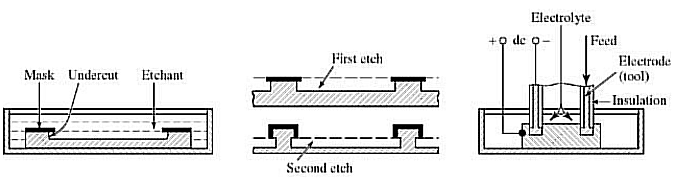
\includegraphics[width = \textwidth]{LavChimiche}
\caption{Modalità di attacco chimico}
\label{fig:LavChimiche}
\end{figure}

Data la natura della lavorazione, si nota che si può avere della corrosione anche al di sotto della maschera. Per cui si formano dei sottosquadri. Tra l'altro, gli stessi, risulteranno non rettilinei ma curvilinei per il fatto che quella superficie rimane esposta per più tempo all'agente corrosivo, a differenza del piano che si vorrebbe lavorare.
Si tratta di un'operazione che può essere ripetuta più volte. Il risultato è una superficie piana.
Il livello di rugosità può essere piuttosto modesto come illustrato in figura \ref{fig:RisLavChimiche}, in virtù del fatto che il materiale può essere polifasico, con diversa velocità di corrosione delle fasi presenti nel materiale.

Parlando delle maschere: ne esistono di diverse forme e materiali. In genere si crea un film di materiale resistente alla corrosione che semplicemente viene tagliato per esporre il materiale da corrodere.
La massima accuratezza può essere ottenuta con il film sensibili alla luce usati nella tecnologia dei semiconduttori.

Un esempio di applicazione sta nei pannelli rinforzati dove viene esposta la maggior parte del materiale coprendo una struttura rinforzante. Ne risulta un materiale particolarmente resistente senza dover saldare un'armatura. Si tratta di applicazioni in cui si ha alto valore aggiunto visto che spesso si spreca molto materiale.

Queste lavorazioni vengono favorite, accelerandole, tramite il controllo della temperatura.
Questo aspetto può essere sfruttato anche per operazioni di sbavatura. Non si creano problemi al restante materiale a patto che la bava sia molto più fine del materiale totale. In modo tale che si scaldi più facilmente di tutto il materiale e risulti più facile attaccarla.

\begin{figure}
\centering
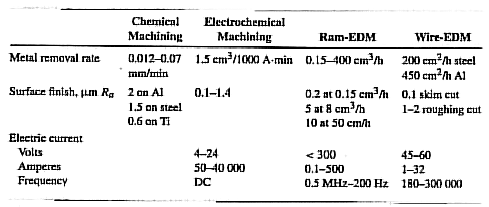
\includegraphics[width = \textwidth]{RisLavChimica}
\caption{Risultati ottenibili con le lavorazioni chimiche}
\label{fig:RisLavChimiche}
\end{figure}

\paragraph{Tranciatura chimica}
La tranciatura chimica viene usata per tagliare lamiere sottili.
Quando la maschera viene ottenuta tramite tecniche fotochimiche, il processo viene chiamato lavorazione fotochimica.


\section{Lavorazioni elettrochimiche}
Vengono sottratti degli atomi (ioni) dal materiale da lavorare considerabile come anodo. Il tutto viene messa in bagno elettrochimico. Viene poi messo un catodo che funge da utensile per captare tali ioni separati dall'anodo.
Entrambi i materiali devono essere conduttori altrimenti tutto ciò non ha senso.
Su alcuni metalli può costituirsi uno strato di ossido, ma può essere facilmente rimosso tramite scintille.
Il funzionamento è illustrato alla figura \ref{fig:LavElettroChim}.

\begin{figure}
\centering
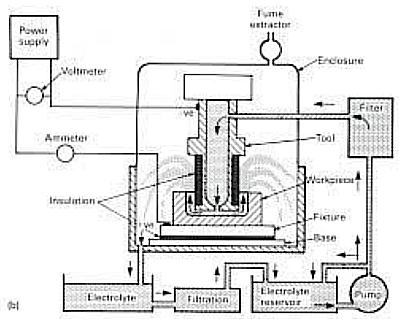
\includegraphics[width = \textwidth]{LavElettroChim}
\caption{Schema generale delle lavorazioni elettrochimiche}
\label{fig:LavElettroChim}
\end{figure}

\subsection{Elettroerosione}
Si tratta di una lavorazione molto importante perché permette di finire gli stampi. Anche se ultimamente sta perdendo dispiego.
Rispetto alla precedente, in cui il liquido è donduttore per chiudere il circuito elettrico. IN queste lavorazioni il liquido è un isolante: impedisce la chiusura del circuito elettrico.

I due elementi sono ad una certa distanza col liquido che fa da isolante. Si avvicina l'elettrodo fino a che l'isolante non riesce a tenere la rigidità elettrica e fa passare una scintilla tra i due elementi.
Sarà la scintilla stessa che permette l'asportazione del materiale.
La lavorazione consiste nei successivo avvicinamenti e allontanamenti dell'utensile e lavorato.
La scintilla vaporizza il materiale asportato, che risolidificherà nel liquido, il quale ha il compito di spostare il più velocemente possibile il solidificato. Altrimenti fungerebbe da conduttore.

Molto importante è l'elettronica di controllo per la corretta esecuzione di tale lavorazione. Infatti queste lavorazioni, che sono molto lente, sono completamente automatizzate: sia per la natura pericolosa della lavorazione che per il corretto funzionamento. Ciò non occupa un operatore per tutta l'operazione.

Il dielettrico: isola, raffredda e sposta i residui. Risulta essenziale che sia in continuo movimento affinché lavori correttamente. Oltretutto deve essere continuamente filtrato per evitare che le particelle asportate rimangono in circolo. 

In termini di finitura, la densità di corrente ha un ruolo importante: da un lato si vorrebbe una densità di corrente elevata per asportare più materiale possibile e accelerare la lavorazione; però ne risente la finitura superficiale che ne risulta peggiore all'aumentare della stessa densità di corrente.
Poiché elettrodo e pezzo non vanno a contatto si ha un \eng{overcut}. Ovvero non c'è la necessità che l'utensile abbia la stessa forma in negativo del pezzo da lavorare. L'elettrodo va comunque dimensionato correttamente proprio per evitare che tale \eng{overcut} sia problematico.
Inoltre l'\eng{overcut} si riduce al diminuire della densità di corrente.
Infatti, in passato si utilizzavano elettrodi consumati per effettuare sgrossature più importanti e poi elettrodi nuovi per migliorare la finitura.
Ad oggi si preferisce effettuare una fresatura come operazione di sgrossatura, mentre si lascia la finitura all'elettroerosione.
In alcune aziende viene addirittura soppiantata da eventuale fresatura con utensili ad inserti CBN. Tale per via dello sviluppo dei materiali superduri come CBN e diamante ove utilizzabile.

Gli elettrodi possono essere consumarsi, in genere sono fatti in rame o grafite, con un rapporto di erosione che va dai $3:1$ del rame fino a $100:1$ della grafite.

\subsection{Elettroerosione a tuffo}
L'elettrodo ha un movimento alternato tra avvicinamento e allontanamento.
Ha la forma che si vuole ottenere in negativo.
\missingfigure{elettroerosione a tuffo}
I dielettrici più usati sono
\begin{itemize}
\item olio dielettrico
\item Eventualmente acqua
\end{itemize}
In qualche caso, l'elettrodo ha movimento laterale ma è una casistica molto rara.

\subsection{Elettroerosione a filo}
\missingfigure{schema elettroerosione a filo}
Si parte da un blocco di materiale e tramite l'elettroerosione a filo si va a scontornare il materiale.
Si realizzano dei fori di forma qualsiasi a pareti ortogonali rispetto al piatto. Il risultato è simile ad una lappatura o tranciatura.

Viene sfruttata questa operazione per realizzare il sistema punzone-matrice per le operazioni di tranciatura.

In questo caso il dielettrico non è in bagno ma viene spruzzato direttamente sul filo, o sul luogo in cui il filo sta tagliando.
Di fatto il sistema diventa analogo alla sega a nastro.
In generale è il portapezzo che si muove con traslazioni planari. Può essere che le spolette abbiano un loro movimento, in quel caso si possono realizzare delle superfici inclinate.

Anche per questa lavorazione c'è il problema dell'\eng{overcut}. 

L'elettroerosione può essere sfruttata anche in altre situazioni: ad esempio la si può sfruttare per realizzare dei fori a qualsiasi profondità di piccola sezione trasversale. Basta realizzare degli elettrodi dedicati.

\section{Lavorazioni con fasci alto contenuto energetico}
\todo{\\Aggiungi dettagli funzionamento generico lavorazioni a fasci energetici}
\subsection{A fascio elettronico}
\missingfigure{Tubo catodico}
Si tratta di una lavorazione effettuata tramite fascio elettronico.
Di solito si tratta di tagli o forature tramite queste lavorazioni.
Per generare il fascio elettronico avviene su tubi catodici.
In genere il tubo catodico è a vuoto spinto per garantire migliore precisione del fascio di elettroni.
Si susseguono una serie di avvolgimenti elettrici che permettono di concentrare e direzionare il fascio elettronico.
Gli elettroni escono dalla camera, vanno ad urtare il materiale lavorato.
L'energia cinetica degli elettroni viene trasformata in energia termica che va a fondere e addirittura a vaporizzare il materiale del lavorato.

Maggiore è il livello di depressione dove il pezzo viene lavorato, maggiore energia viene trasportata sul pezzo. Altrimenti, le molecole presenti a pressione atmosferica deviano gli elettroni del fascio deviandoli dal punto di lavorazione.

Dunque è altrettanto importante la sessione di pompaggio a vuoto del tubo catodico o pistola elettronica. Ciò richiede del tempo, per cui a inizio lavorazione si decide quanto vuoto realizzare dentro la pistola. Più vuoto implica maggiore energia trasmessa ma maggior tempo ciclo.

Queste lavorazioni vengono spesso utilizzate per realizzare delle filiere per materiali polimerici.

\subsection{Taglio Laser}
\missingfigure{Taglio laser}
Il funzionamento non è troppo diverso dalla lavorazione precedente, però si sfruttano emissioni di luce laser per tagliare il materiale.
Il vantaggio è che non c'è la necessità di concentrare elettroni ma fotoni.
Ciò non viene influenzato dalla presenza di altre particelle presenti in atmosfera.

In più il laser è estremamente preciso in quanto il cono in cui vengono sparati gli elettroni è molto piccolo.
In più essendo che la luce laser è concorde e monocromatica, rende lo sfruttamento di tale tecnologia più efficace.
Le sostanze che vengono utilizzate per produrre luce laser sono ben definite e conosciute.
Inoltre, essendo che è possibile orientare il fascio di raggi laser, è possibile lavorare anche in punti nascoste.

Come primo materiale si è sfruttato il rubino, che viene utilizzato per sistemi di puntamento. Infatti l'energia concentrabile tramite rubino non è eccessivamente elevata, ma si può estendere per lunghezze considerevoli.

la dimensione del punto che si va a realizzare dipende da:
\begin{itemize}
\item Lunghezza d'onda: più è alta più si riesce a controllare lo spot.
\item L'ottica: migliore è l'ottica e più energia si riesce a concentrare energia.
\end{itemize}
Industrialmente parlando, viene utilizzata l'anidride carbonica come materiale emettitore. La luce emessa è nell'intervallo degli infrarossi lontani: alta lunghezza d'onda e bassa frequenza.
Perciò la concentrazione non è molto alta, però si raggiungono potenze nell'ordine dei $40\unit{\kW}$ con efficienza del $15\%$ che sembra poco ma nel campo dei laser è considerevole.
Si può direzionare il fascio attraverso degli specchi che riescono a riflettere la specifica lunghezza d'onda. Non si tratta di specchi convenzionali.

Altro materiale emettitore è il \texttt{Nd:YAG}, produce degli infrarossi vicini: si hanno migliori concentrazioni di energia ma con valori di potenza di molto inferiori rispetto al precedente. Dunque non si raggiungono gli stessi valori di temperatura raggiunte con la $CO_2$.
Di certo, essendo più concentrata l'energia si può trasmettere a distanze maggiori. In più con opportune ottiche si può suddividere in più fasci.

Altra casistica è quello del \texttt{laser a eccimeri}. Si ha una lunghezza d'onda molto piccola ed alta frequenza, arrivando allo spettro degli ultravioletti. 
Ciò permette di avere una grandissima precisione, infatti vengono impiegati perla realizzazione di pezzi in minuteria, in chirurgia.
Si possono utilizzare in modalità continua o pulsata.

In generale per le lavorazioni a taglio laser non ha controllo della profondità di lavorazione. Allora si utilizzano per realizzare dei fori passanti.
Spesso viene fornito ossigeno per aumentare l'assorbimento di energia.
Ciò peggiora la finitura superficiale. 
Viste le temperature raggiunte si possono lavorare dei materiali altofondenti. Non c'è il problema di mettere sottovuoto il pezzo.

la lunghezza d'onda influisce sul diametro minimo del più piccolo foro realizzabile:
$0.5\unit{\mm}$ per la $CO_2$, fino ad arrivare al $1\unit{\um}$ per il laser ad eccimeri.

\subsection{Taglio al plasma}
\begin{quote}
Cos'è il plasma?
\end{quote}
Si tratta di un gas ionizzato, viene definito così perché le proprietà fisiche del plasma sono considerevolmente differenti dallo stato di gas per via delle ionizzazioni delle particelle.
Viene usato in industria per tagliare lamiere ed effettuare saldature ad alta velocità per via delle più alte temperature raggiunte.
Il taglio al plasma ha una finitura peggiore di quelle ottenibili tramite laser.
\missingfigure{taglio al plasma}

\subsection{Taglio al cannello ossiacetilenico}
\missingfigure{Taglio ossiacetilenico}
Si sfrutta una fiamma ossiacetilenica per scaldare il materiale per tagliare lamiere. Anche in questo caso si hanno delle finiture peggiori delle precedenti. Infatti si preferisce usarlo per effettuare delle saldature.

\section{Taglio ad acqua}
Si usa l'energia meccanica generata da un getto d'acqua contenente delle particelle abrasive.
Non è una vera e propria lavorazione non convenzionale per via del fatto che in questo caso si sta sfruttando l'energia cinetica dell'acqua o particelle abrasive per rimuovere il materiale.

A differenza delle precedenti non provoca il riscaldamento del materiale.
Si può usare anche per materiali particolarmente fragili come vetro e marmo.
Non è una lavorazione molto efficiente per via della molta energia da imprimere all'acqua. Inoltre è particolarmente rumorosa.